\documentclass[12pt,leqno,fleqn]{beamer}
\usepackage[utf8]{inputenc}
\usepackage[english, russian]{babel}
\usepackage[OT1]{fontenc}
\usepackage{amsmath}
\usepackage{amsfonts}
\usepackage{amssymb}
\usepackage{graphicx}
\usepackage{textpos}
\usetheme{Malmoe}
\author{Artyom Aleksyuk}
\title{IPv6}
\institute{KSPT ICC SPbSTU}
%\subtitle{Подзаголовок}
\begin{document}
\maketitle

\setlength{\TPHorizModule}{1cm} % Horizontale Einheit
\setlength{\TPVertModule}{1cm} % Vertikale Einheit

%--------------------------------------------------------------

\begin{frame}
\frametitle{IP overview}
\begin{itemize}
\item \textbf{IP} (Internet Protocol) – an L3 protocol in the ISO/OSI model
\item An intermediate protocol, however very important
\item Relays data across network boundaries
\item Negotiates different physical layer technologies
\item Establishes the Internet
\end{itemize}
\end{frame}

%--------------------------------------------------------------

\begin{frame}
\frametitle{IP address}
\begin{itemize}
\item Each host (a network participant, except L2/L1 devices) has an unique IP address
\item Usually you don’t use it directly (\textit{and there’s a reason for that!})
\item Nonetheless it's a neccesary part of a communication process
\item For example, you can’t call the phone if you don’t know it’s number
\end{itemize}
\end{frame}

%--------------------------------------------------------------

\begin{frame}
\frametitle{IP address}
\begin{itemize}
\item IPv4 – still 96\% of the traffic
\item Addresses are 32 bit sized
\item $2^{32} \approx 4$ billion addresses
\item It’s a lot?
\end{itemize}
\end{frame}

%--------------------------------------------------------------

\begin{frame}
%\frametitle{IP address}

\begin{picture}(320,250)
\put(160,140){\includegraphics[height=4cm]{pos.png}}
\put(-60,0){\includegraphics[height=5.3cm]{FP.png}}
\put(100,0){\includegraphics[height=5cm]{sensors.jpg}}
\put(0,240){\begin{minipage}[t]{0.4\linewidth}
{\begin{itemize}
\item Feature phones
\item POS terminals
\item Sensors
\item It’s a lot? \textbf{Nope.}
\end{itemize}}
\end{minipage}}
\end{picture}



\end{frame}

%--------------------------------------------------------------

\begin{frame}
\frametitle{IPv4 address exhaustion}
\includegraphics[keepaspectratio=true,width=1\textwidth]{ipv4_stat.png}
\end{frame}

%--------------------------------------------------------------

\begin{frame}
\frametitle{Popular solutions}
\begin{itemize}
\item Two popular solutions: Proxy and NAT
\item Like a call center: one number, many phones.

\vspace{8mm}
\includegraphics[keepaspectratio=true, width=0.4\textwidth]{image5.jpeg}
\hspace{8mm}
\includegraphics[keepaspectratio=true, width=0.4\textwidth]{image6.jpeg}

\end{itemize}
\end{frame}

%--------------------------------------------------------------

\begin{frame}
\frametitle{What’s the problem?}
\begin{itemize}
\item Relies on higher-level protocols
\item Slower than a simple routing
\item The main drawback: an address is not unique anymore.
\item Cannot accept incoming connections
\item Often called a “grey” IP address
\item Conclusion: an IPv4 address is just a bunch of numbers nowadays, that’s the reason why you don’t use it directly.

\end{itemize}
\end{frame}

%--------------------------------------------------------------

\begin{frame}
\frametitle{DON'T SLEEP!}
\includegraphics[scale=0.25]{kitty.jpg}
\end{frame}

%--------------------------------------------------------------

\begin{frame}
\frametitle{IPv6}
\begin{itemize}
\item Since 1996
\item $2^{128}$ addresses, or approx. $3.4 \cdot 10^{38}$
\end{itemize}

\includegraphics[keepaspectratio=true, height=0.35\textheight]{Ipv4_address.pdf}

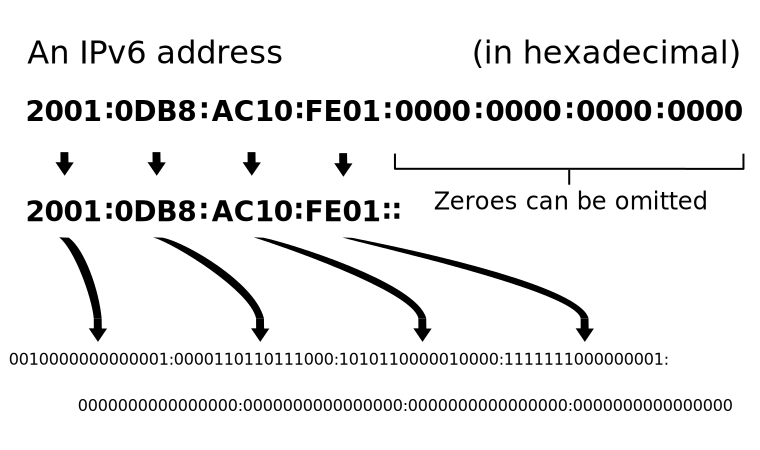
\includegraphics[keepaspectratio=true, height=0.35\textheight]{Ipv6_address.pdf}
\end{frame}

%--------------------------------------------------------------

\begin{frame}
\frametitle{Minor changes}
\begin{itemize}
\item ARP {\large $\Rightarrow$} NDP
\item Broadcast via multicast
\item DHCP {\large $\Rightarrow$} SLAAC
\item IPv6 routers do not perform fragmentation
\item TTL {\large $\Rightarrow$} Hop limit
\end{itemize}
\end{frame}

%--------------------------------------------------------------

\begin{frame}
\frametitle{IPv6 adoption rate}
\includegraphics[keepaspectratio=true,width=1\textwidth]{adoption_rate.png}
\end{frame}

%--------------------------------------------------------------


\end{document}
